% Appendix D: Illustrative UMAP Atlas of Selected Subfields

This appendix provides an illustrative atlas of selected subfield-level UMAP projections.
The panels are not used to compute morphology metrics, assign clusters, measure distances,
or support quantitative claims. They are included as visual diagnostics to make selected
paper-cloud morphologies interpretable at the document-cloud level. All quantitative claims
in the thesis remain based on metrics computed in the original SPECTER2 embedding space.
Because each panel is a separate subfield-specific UMAP projection, axes, distances, shapes,
and density scales should not be compared across subfields.

The atlas maps were generated separately for each selected subfield from the row-aligned
SPECTER2 analysis matrix, using main-analysis records from 2000--2024 and at most
10,000 papers per subfield. The per-subfield UMAP routine used cosine distance with
\texttt{n\_neighbors = 30}, \texttt{min\_dist = 0.05}, \texttt{random\_state = 42}, and
\texttt{low\_memory = true}. The density panel is a \texttt{smooth\_hist} rendering:
a 150-by-150 two-dimensional histogram over the displayed UMAP coordinates, smoothed
with a Gaussian filter of \(\sigma = 3.0\), clipped at the 99th percentile of positive
density values, and drawn with \texttt{viridis}. The atlas-generation script reads the
stored SPECTER2 matrix directly; no additional vector-normalization step is exposed in
that plotting routine. These settings are reported for reproducibility only, and the
resulting coordinates are not used for quantitative measurement.

The selected cases are not the visually prettiest maps in isolation. They are chosen because
they connect to recurring empirical themes in the thesis: atypical profiles, dispersed
physical-science structure, compact or separated local organization, computer-science novelty,
and broad material-science morphology. These figures are intended as visual companions to the
metric-based interpretation in Chapters 6--9. The six cases cover an atypical social-science
profile, a dispersed physical-science cloud, a compact life-science structure with a separated
component, two computer-science novelty cases, and a broad material-science morphology.

% Figure 1: Human Factors and Ergonomics
\begin{figure}[p]
    \centering
    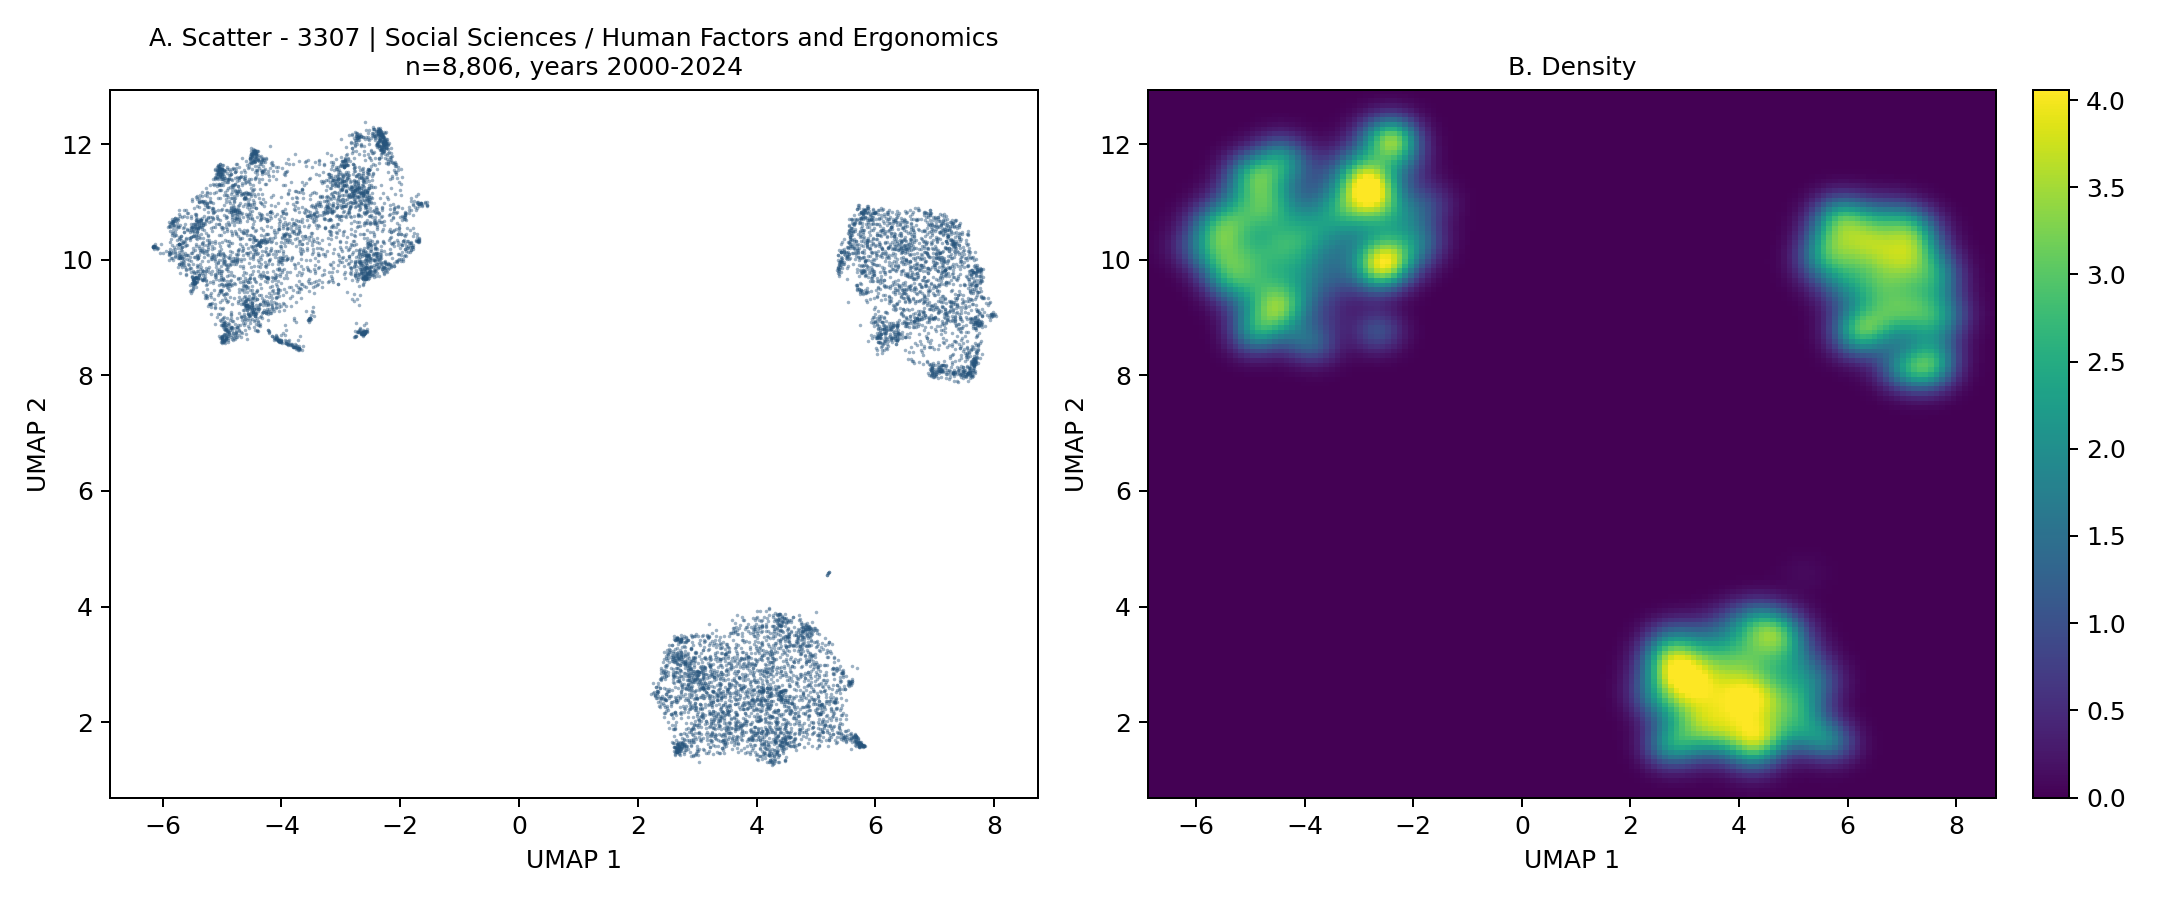
\includegraphics[width=\textwidth]{figures/umap_atlas/fig_d_umap_human_factors_ergonomics.png}
    \caption[Illustrative UMAP atlas: Human Factors and Ergonomics]{%
        Illustrative UMAP atlas: Human Factors and Ergonomics.
        The separated paper-cloud components make this case visually useful for interpreting
        the atypical profile behavior discussed in the thesis. The projection is illustrative
        only; quantitative metrics are computed in the original SPECTER2 space.}
    \label{fig:umap_atlas_human_factors}
\end{figure}

% Figure 2: Nuclear and High Energy Physics
\begin{figure}[p]
    \centering
    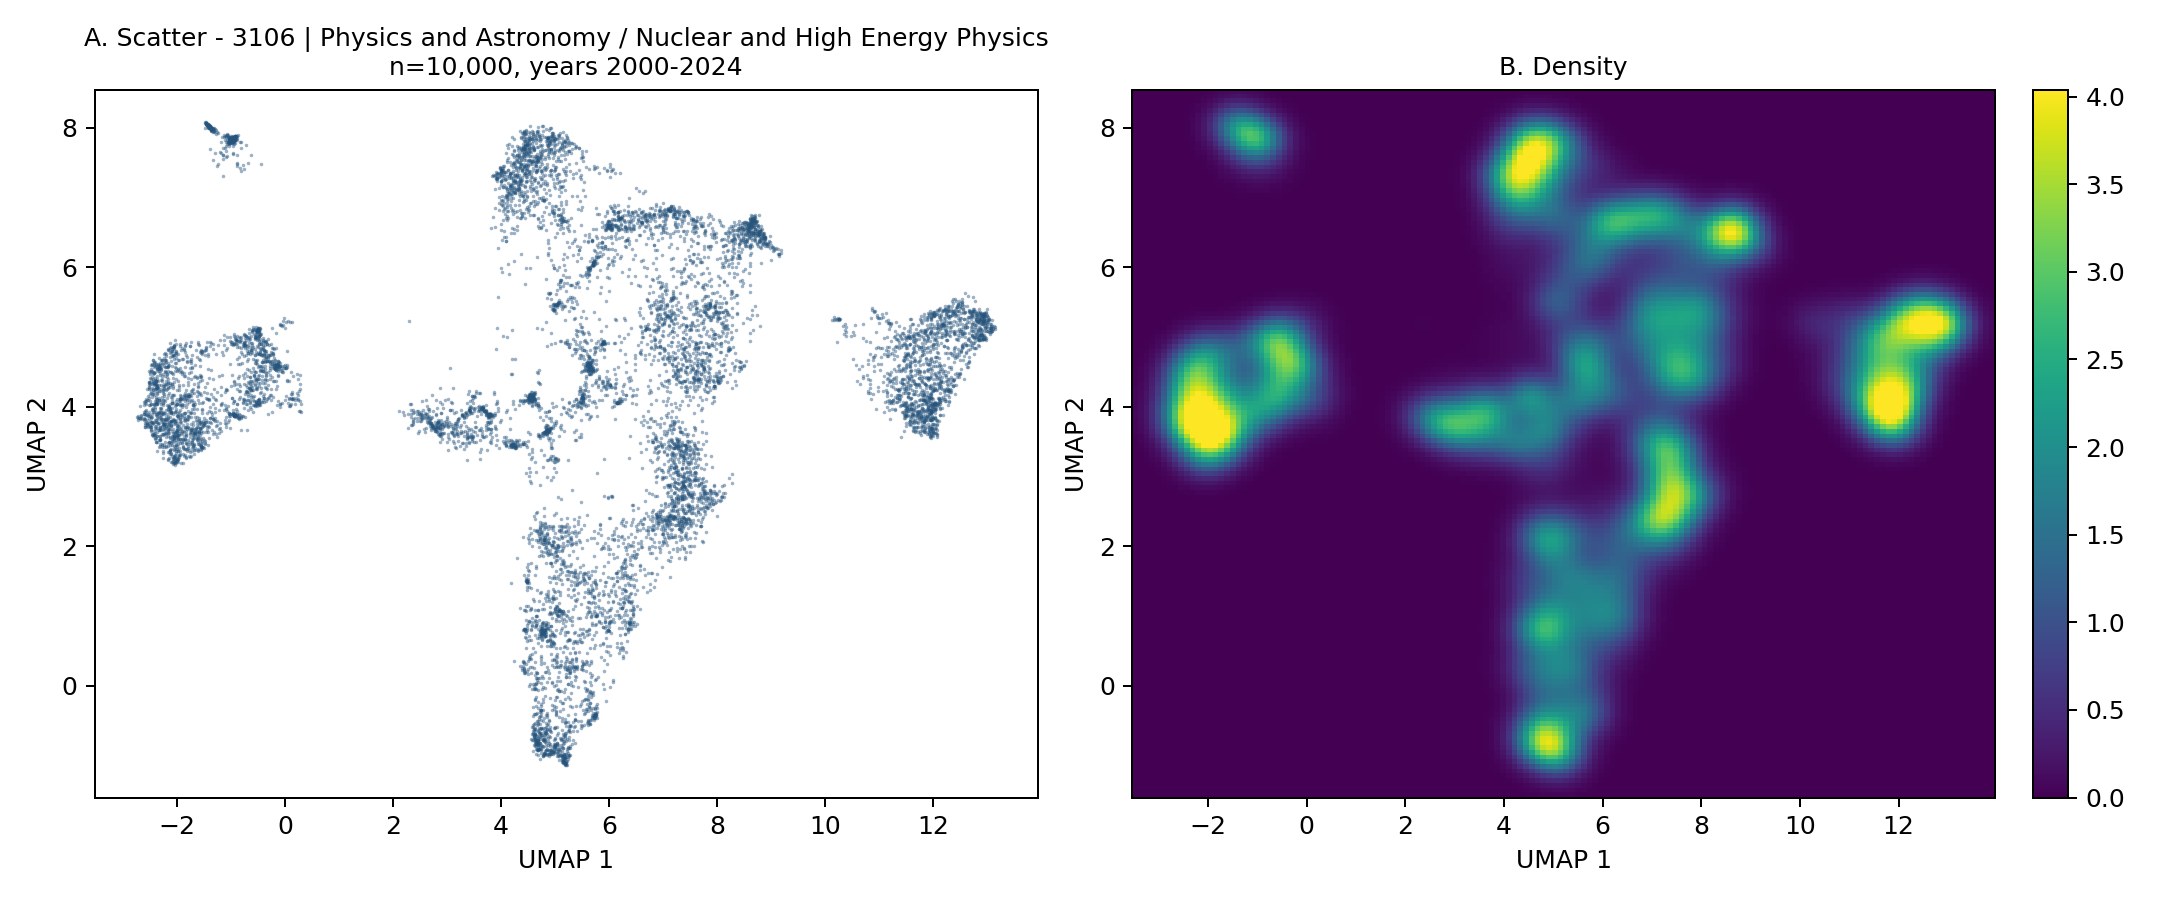
\includegraphics[width=\textwidth]{figures/umap_atlas/fig_d_umap_nuclear_high_energy_physics.png}
    \caption[Illustrative UMAP atlas: Nuclear and High Energy Physics]{%
        Illustrative UMAP atlas: Nuclear and High Energy Physics.
        The fragmented visual structure provides an example of a dispersed physical-science
        paper cloud. UMAP is used only as a subfield-level visualization and not as a
        measurement space.}
    \label{fig:umap_atlas_nuclear_physics}
\end{figure}

% Figure 3: Applied Microbiology and Biotechnology
\begin{figure}[p]
    \centering
    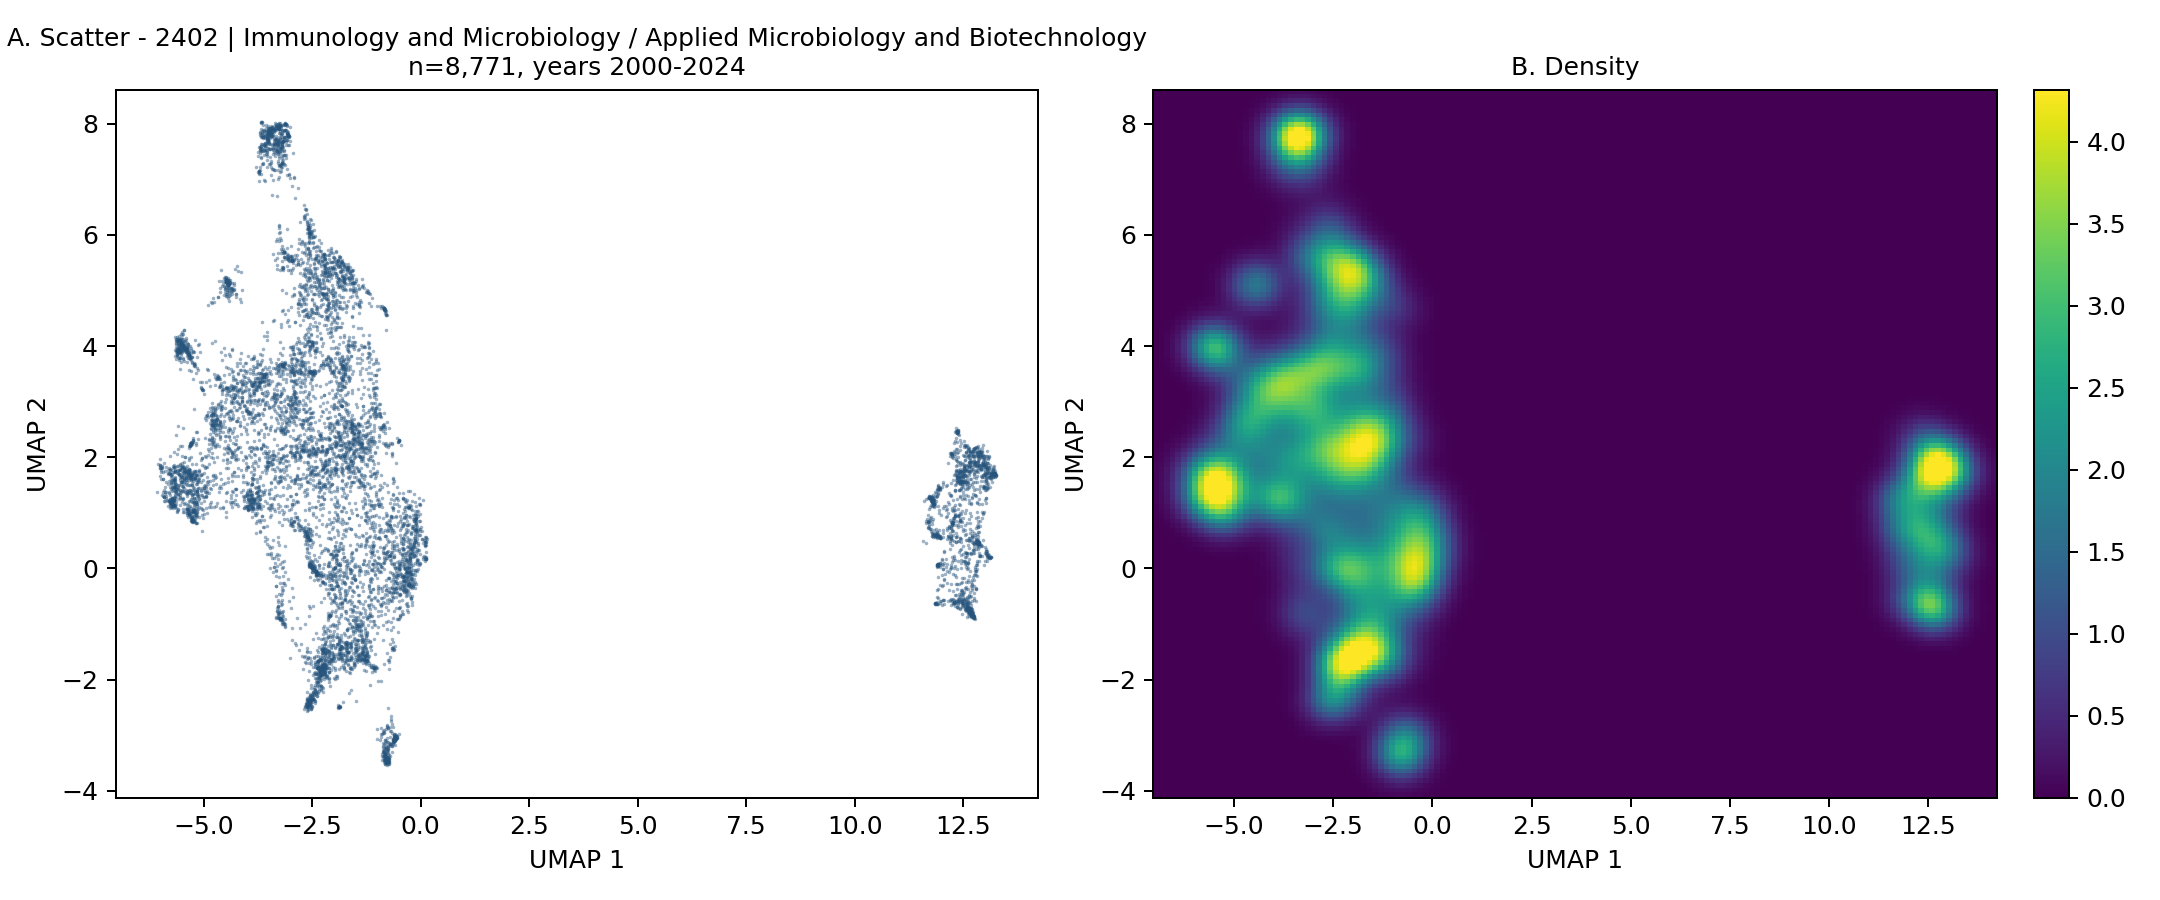
\includegraphics[width=\textwidth]{figures/umap_atlas/fig_d_umap_applied_microbiology_biotechnology.png}
    \caption[Illustrative UMAP atlas: Applied Microbiology and Biotechnology]{%
        Illustrative UMAP atlas: Applied Microbiology and Biotechnology.
        The map illustrates a dense main region together with a separated component,
        making the case useful for visualizing local organization beyond a single centroid.
        The projection is illustrative only.}
    \label{fig:umap_atlas_applied_microbiology}
\end{figure}

% Figure 4: Computer Vision and Pattern Recognition
\begin{figure}[p]
    \centering
    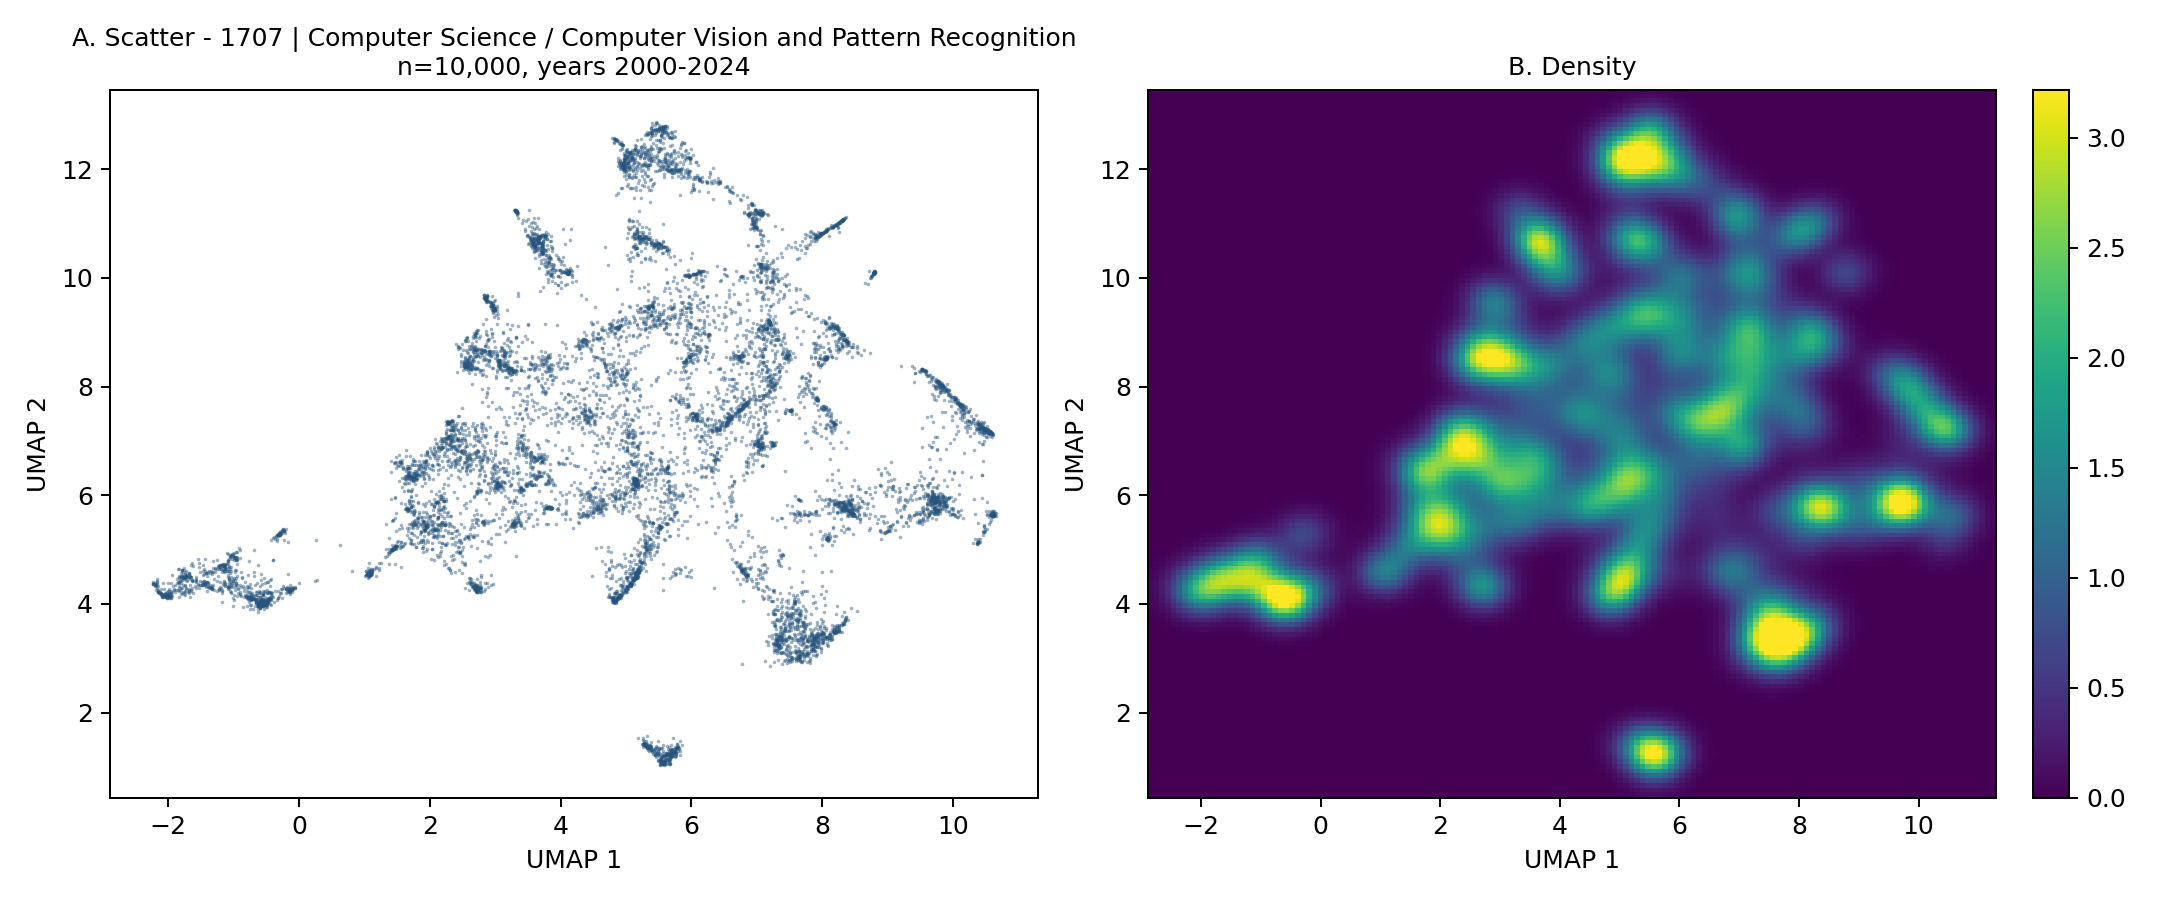
\includegraphics[width=\textwidth]{figures/umap_atlas/fig_d_umap_computer_vision_pattern_recognition.png}
    \caption[Illustrative UMAP atlas: Computer Vision and Pattern Recognition]{%
        Illustrative UMAP atlas: Computer Vision and Pattern Recognition.
        The panel provides a visually rich Computer Science example connected to the thesis
        discussion of novelty and movement. The projection is not used to define clusters
        or distances.}
    \label{fig:umap_atlas_computer_vision}
\end{figure}

% Figure 5: Signal Processing
\begin{figure}[p]
    \centering
    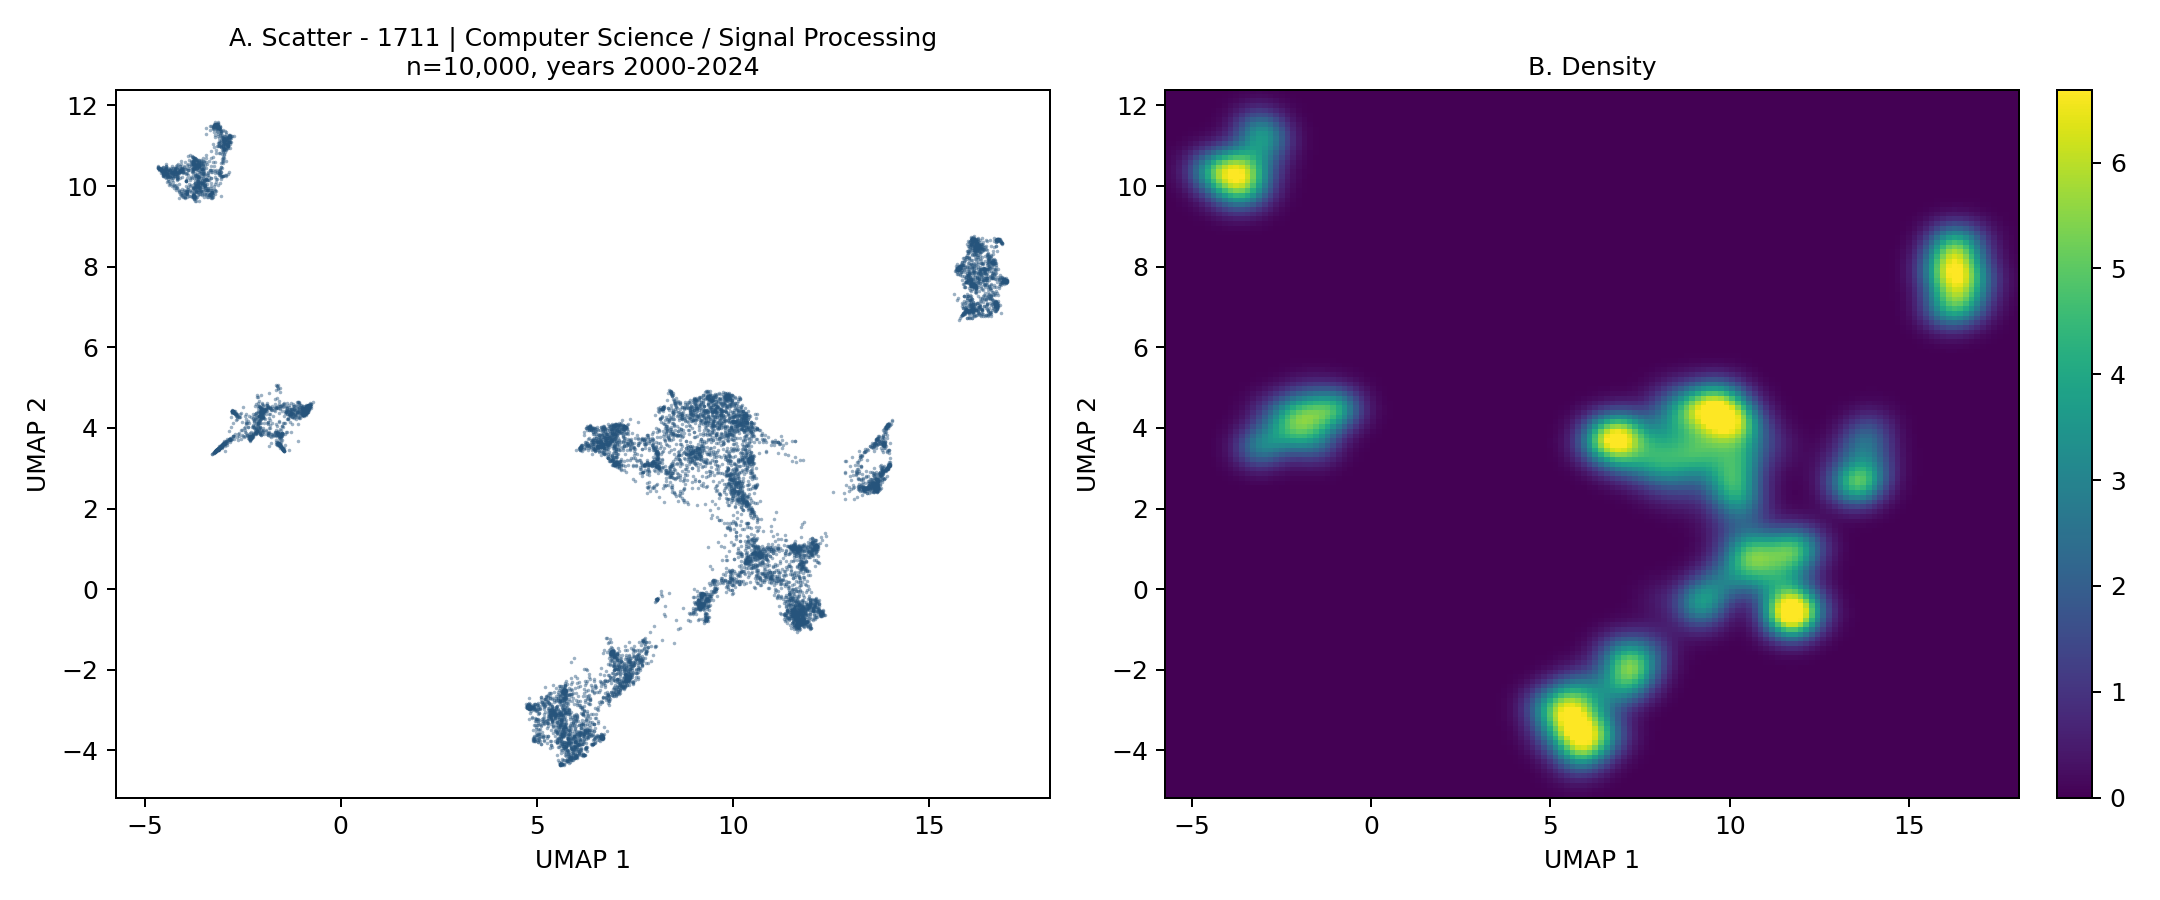
\includegraphics[width=\textwidth]{figures/umap_atlas/fig_d_umap_signal_processing.png}
    \caption[Illustrative UMAP atlas: Signal Processing]{%
        Illustrative UMAP atlas: Signal Processing.
        The separated components make this a useful visual companion to the temporal and
        novelty-oriented Computer Science cases. The projection is illustrative only and
        should not be compared geometrically with other panels.}
    \label{fig:umap_atlas_signal_processing}
\end{figure}

% Figure 6: General Materials Science
\begin{figure}[p]
    \centering
    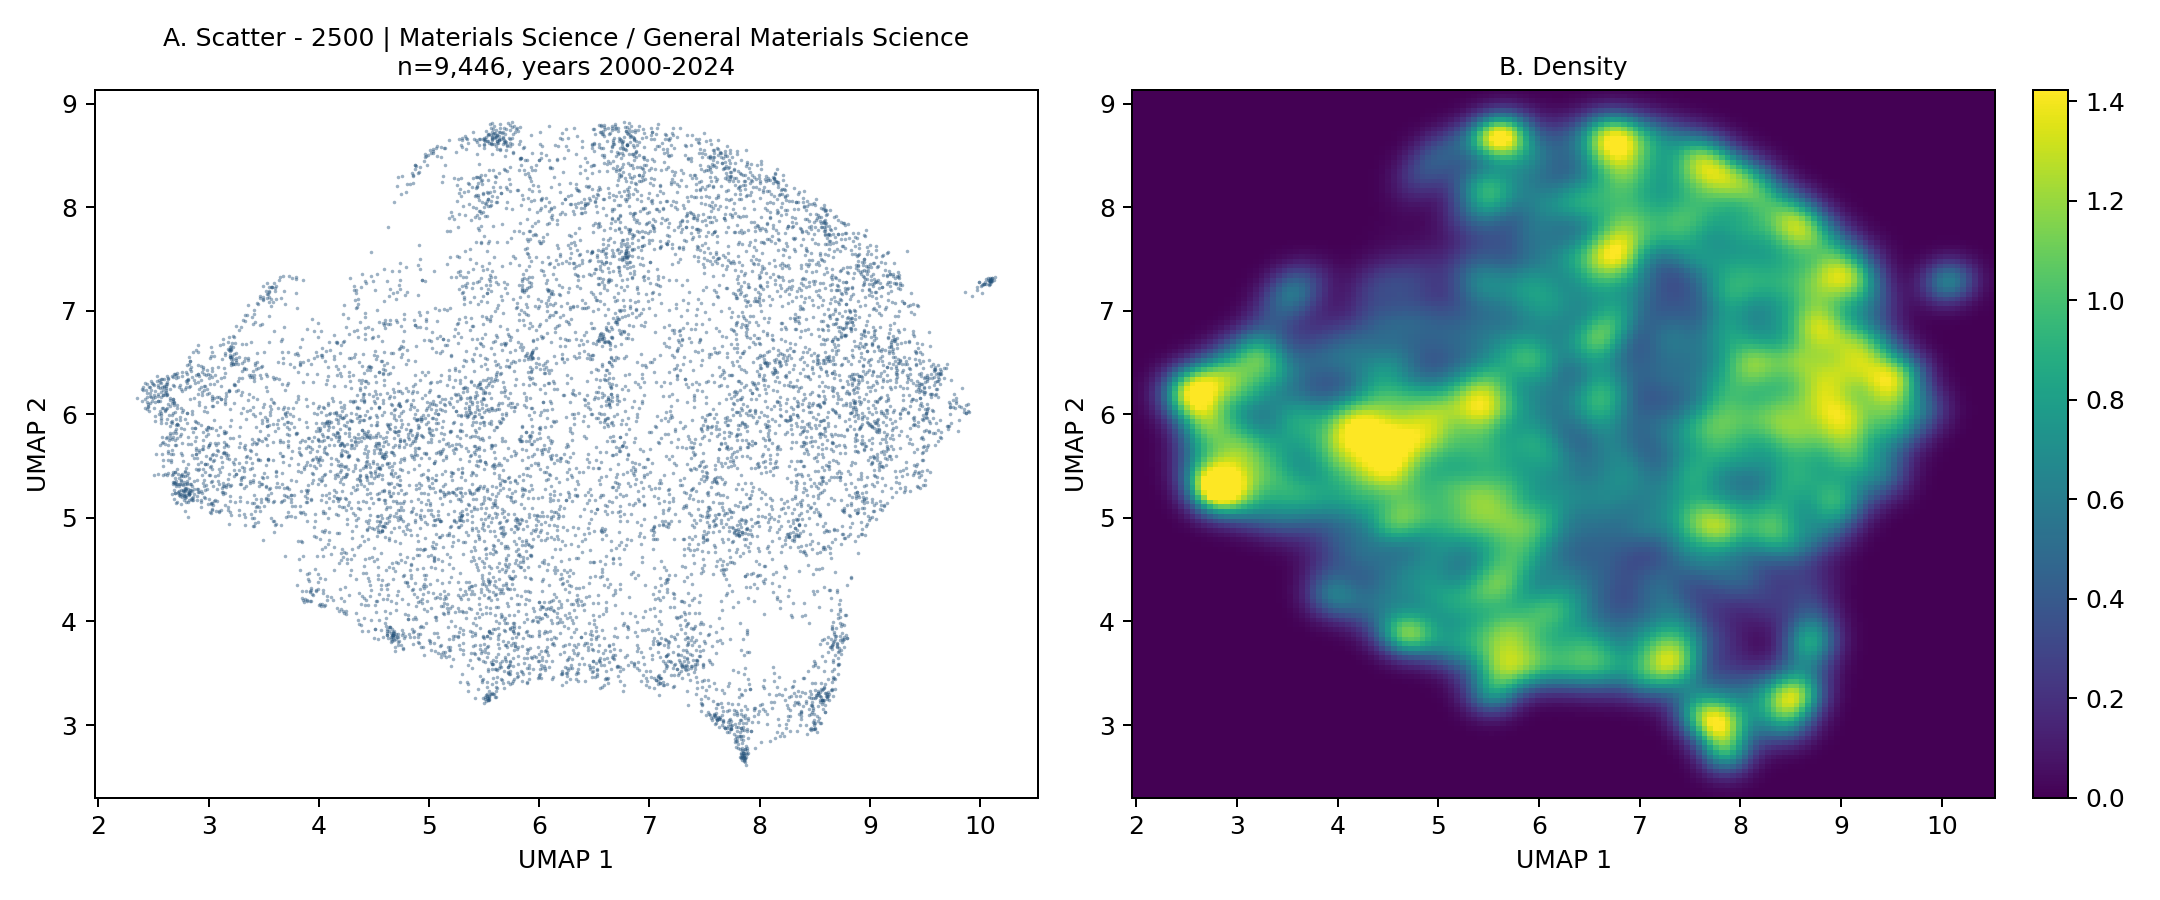
\includegraphics[width=\textwidth]{figures/umap_atlas/fig_d_umap_general_materials_science.png}
    \caption[Illustrative UMAP atlas: General Materials Science]{%
        Illustrative UMAP atlas: General Materials Science.
        The broad continuous cloud provides a contrast to the more fragmented examples in the
        atlas and illustrates why morphology is not reducible to a single centroid. Quantitative
        interpretation remains based on original-space metrics.}
    \label{fig:umap_atlas_general_materials}
\end{figure}
